\documentclass[tikz,border=2]{standalone}
\usetikzlibrary{shadows,arrows,shapes,positioning,calc,backgrounds,fit,automata}
\begin{document}
%%%%%%%%%%%%%%%%%%%%%%%%%%%%%%%%%%%%%%%
% Define the layers to draw the diagram
\pgfdeclarelayer{bg}
\pgfsetlayers{bg,main}
%%%%%%%%%%%%%%%%%%%%%%%%%%%%%%%%%%%%%%%
% colors
\definecolor{myBlue}{HTML}{0060AD}
\definecolor{myRed}{HTML}{DD181F}
%%%%%%%%%%%%%%%%%%%%%%%%%%%%%%%%%%%%%%%
\newcommand{\vanish}[1]{}
%\newcommand{\vanish}[1]{#1}

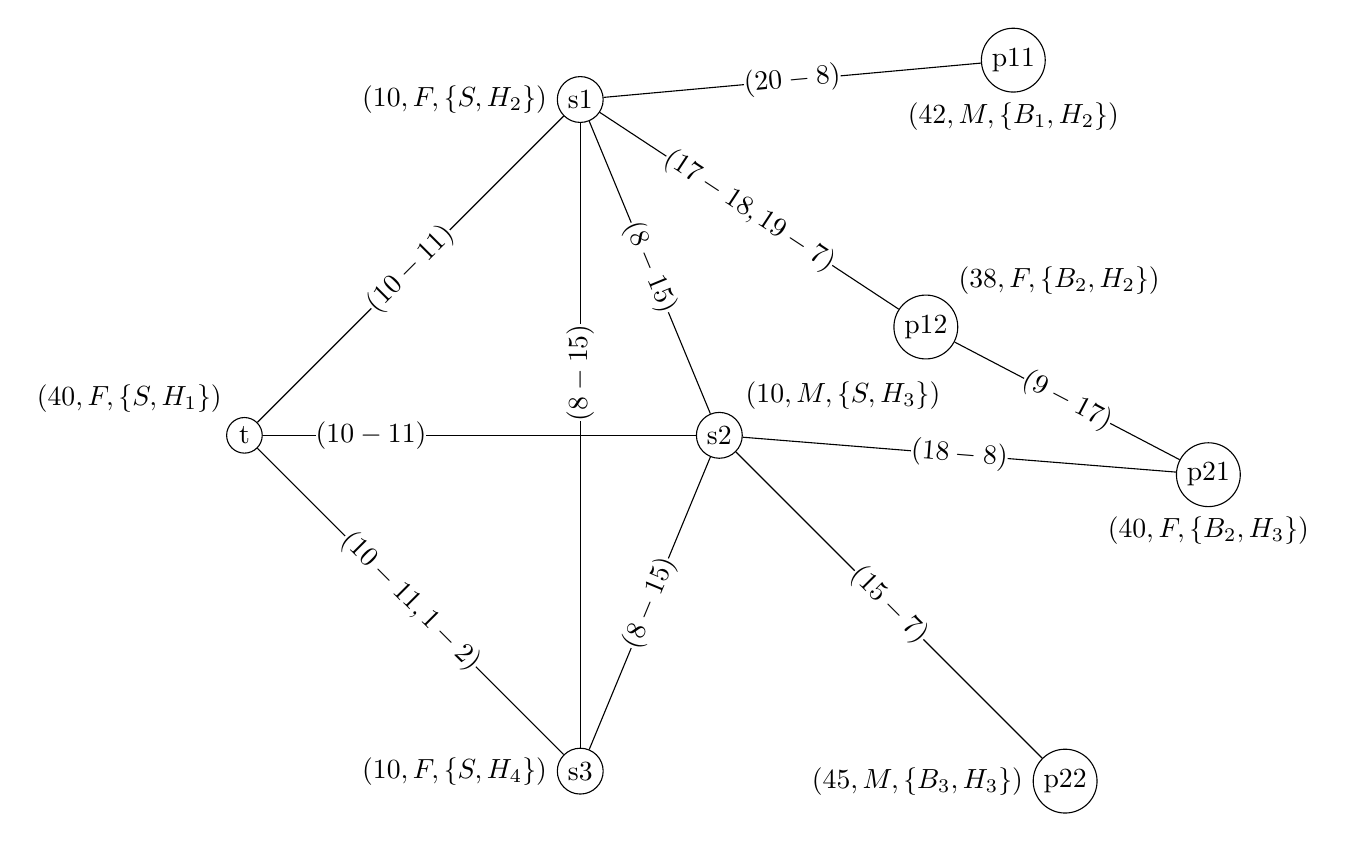
\begin{tikzpicture}
[node distance=5.5cm,
bend angle=15,
subdue/.style={draw=black!30},
vertex/.style={shape=circle,inner sep=2pt},
treevertex/.style={shape=circle,inner sep=2pt,draw=black},
accepting/.append style={draw=myBlue,fill=myBlue},
infected/.style={shape=circle,draw=black,inner sep=2pt,fill=brown},
%
myedge/.style={},
elabel/.style={fill=white,inner sep=0pt},
dedge/.style={dashed,>=latex', shorten >=.0pt, black!90, shorten <=.0pt}]
%
%
\node (t) [vertex,draw,label=above left:{$(40,F,\{S,H_1\})$}] at (0,0) {\vanish{t}};
\node (s1) [vertex,draw,above right=of t,label=left:{$(10,F,\{S,H_2\})$}] {\vanish{s1}};
\node (s2) [vertex,draw,right=of t,label=above right:{$(10,M,\{S,H_3\})$}] {\vanish{s2}};
\node (s3) [vertex,below right=of t,draw,label=left:{$(10,F,\{S,H_4\})$}] {\vanish{s3}};
\node (p11) [vertex,draw,right of=s1,label=below:{$(42,M,\{B_1,H_2\})$},shift={(0,.5)}] {\vanish{p11}};
\node (p12) [vertex,draw,below right of=s1,shift={(.5,1)},label=above
right:{$(38,F,\{B_2,H_2\})$}] {\vanish{p12}};
\node (p21) [vertex,right=of s2,draw,label=below:{$(40,F,\{B_2,H_3\})$},shift={(0,-.5)}] {\vanish{p21}};
\node (p22) [vertex,below right=of s2,draw,label=left:{$(45,M,\{B_3,H_3\})$}] {\vanish{p22}};
%
\path (t) edge[myedge] node[sloped,elabel]{$(10-11)$} (s1);
\path (t) edge[myedge] node[sloped,elabel,pos=0.25]{$(10-11)$} (s2);
\path (t) edge[myedge] node[sloped,elabel]{$(10-11,1-2)$} (s3);
%
\path (s1) edge[myedge] node[sloped,elabel]{$(8-15)$} (s2);
\path (s3) edge[myedge] node[sloped,elabel,pos=.6]{$(8-15)$} (s1);
\path (s2) edge[myedge] node[elabel,sloped]{$(8-15)$} (s3);
%
\path (s1) edge[myedge] node[sloped,elabel]{$(20-8)$} (p11);
\path (s1) edge[myedge] node[sloped,elabel]{$(17-18,19-7)$} (p12);
%
\path (s2) edge[myedge] node[sloped,elabel]{$(18-8)$} (p21);
\path (s2) edge[myedge] node[sloped,elabel]{$(15-7)$} (p22);
%
\path (p12) edge[myedge] node[sloped,elabel]{$(9-17)$} (p21);
%
%% \draw[myedge] (v2) -- (v3);
%% %
%% \draw[myedge] (v3) -- (v4);
%% \draw[myedge] (v3) -- (v5);
%% \draw[myedge] (v3) -- (v6);
%% %
%% \draw[myedge] (v4) -- (v5);
%% %
%% \draw[myedge] (v5) -- (v6);
%% %
%% \draw[myedge] (v6) -- (v7);
%% %%
\end{tikzpicture}
{}
\end{document}
